\section{Zielsetzung}
\label{sec:Ziel}
Ziel des Versuchs ist die Untersuchung der temperaturabhängigen Viskosität von destilliertem Wasser mittels eines Kugelfallviskosimeters nach Höppler.


\section{Theorie}
\label{sec:Theorie}
Bei einem Kugelfallviskosimeter nach Höppler wird in ein mit der zu
untersuchenden Flüssigkeit gefülltes Rohr eine nur geringfügig kleinere
Kugel eingeführt und das Rohr anschließend aufgerichtet, sodass die Kugel
zu fallen beginnt, wobei das Rohr leicht schräg gehalten wird, damit die Kugel
an der Wand entlang gleitet und Stöße vermieden werden
(siehe Abb. \ref{fig:Viskosimeter}). Es bildet sich hierbei ein Gleichgewicht
zwischen Gravitationskraft, Auftriebskraft und Bremskraft aus, weshalb die Kugel
 mit konstanter Geschwindigkeit fällt. Da der geringe Rohrdurchmesser zu
 laminaren Strömungen führt, tritt als Bremskraft die \textit{Stokessche Reibung}
 auf. Da diese von der Viskosität $\eta$ abhängt, kann man über die Fallzeit auf
 diese schließen.
Es gilt die empirische Formel

\begin{equation}
  \eta = K \left(\rho_K - \rho_{Fl}\right) \cdot t.
  \label{eqn:eta}
\end{equation}
Hierbei bezeichnet $\rho_K$ die Dichte der verwendeten Kugel, $\rho_{Fl}$
dementsprechend die Dichte der verwendeten Kugel und $K$ eine Apparaturabhängige
Konstante, die Fallhöhe und Kugelgröße beinhaltet. Da unter anderem die Dichten
temperaturabhängig sind, gilt dies auch für die Viskosität.
Für Flüssigkeiten gilt hierfür meist die \textit{Andradesche Gleichung}:
\begin{equation}
  \eta(T) = A \, \symup{exp}(B/T).
  \label{eqn:eta(T)}
\end{equation}

\begin{figure}
  \centering
  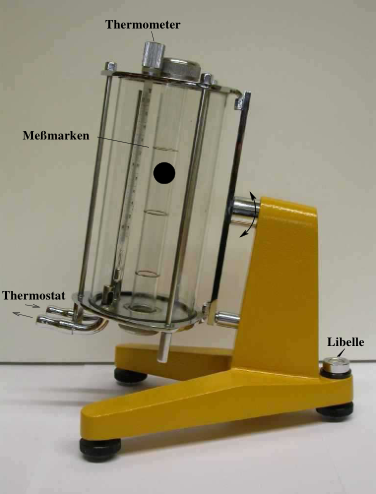
\includegraphics[height=7cm]{./logos/Viskosimeter.PNG}
  \caption{Kugelfallviskosimeter nach Höppler. Hier zu erkennen ist, dass das Fallrohr umschließende Wasserbad zur Temperaturregelung. \cite{Anleitung}}
  \label{fig:Viskosimeter}
\end{figure}
